
\chapter{Platform design}
\label{sec:ch3_platform}

In this chapter, the hardware design processes are outlined based on the user requirements and technical specifications given in Chapter \ref{ch:ch3}. This chapter begins with a description of the mechanical features showing how the design accommodates the electronic subsystems while meeting the functional requirements outlined in Table \ref{tab:hard_funcreqsl}. This chapter then shows the electronic components selected for each subsystem and how they affect the overall system. Finally, this chapter will conclude with the final design considerations for the buoy. \par 

Son and Vorajee in 2018 performed initial concept work for the buoy, which strongly influenced the current design choices for this device. Furthermore, MacHutchon designed the original buoy with modifications by Verrinder to accommodate the buoy. Verrinder designed the physical enclosure and electronic hardware subsystems for the first (V1) and second (V2) versions of the buoy with further design contributions from Jacobson (V1, V2), Cloete (V1) and Pead (V2).
\section{Mechanical features}

The mechanical design for the system falls outside the scope of this project. However, it forms an integral part in protecting the electronics against sea ice dynamics, strong wave activity and freezing. This subsystem consists of two parts: 

\begin{enumerate}
	\item Buoy stand
	\item Enclosure
\end{enumerate}


\subsection{Buoy Stand}

The principle goal of the stand is to anchor the device to the ice floe and protect it from the harsh environment. A buoy stand was designed by K MacHutchon with modification from R. Verrinder and was constructed by the University of Cape Town's Mechanical Engineering Workshop to satisfy this requirement. The stand is shown in Figure \ref{fig:stand} and is 1.2 m tall with a width of 0.71 m. The stand has a cylindrical cradle at the top where the device will be placed. A screw hole in the side of the cradle allows the buoy to be fastened to the stand to prevent it from falling out during deployment. The base of the stand is pyramid shaped with metal spikes to anchor the system to an ice floe. Due to the height of the stand, the system may be susceptible to tipping. This has been overcome by constructing the base to be heavier than the top thereby lowering the centre of gravity. The stand was originally designed for the Trident buoys. However, this design has been modified by increasing the radius of the housing. 

\begin{figure}[H]
	\centering
	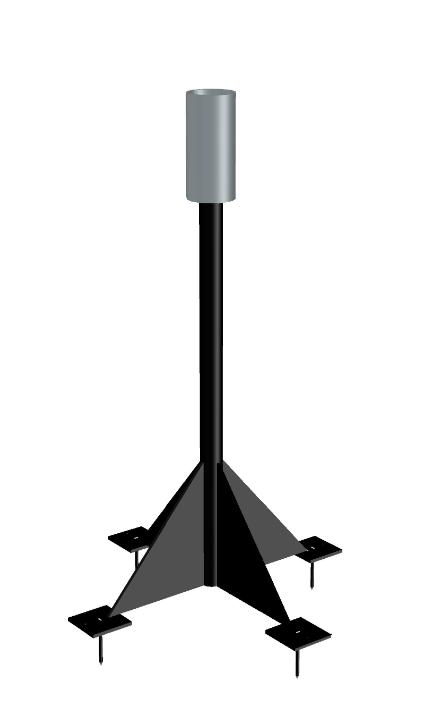
\includegraphics[height = 0.5\textheight]{buoy_stand.PNG}
	\caption{Diagram of the buoy stand for the SHARC buoy. The stand consists of stainless steel and painted mild steel to withstand the climate of the Southern Ocean and stop the stand from rusting. A cradle at the top of the stand houses the buoy and secures it to the stand via a screw. The buoy stand elevates the electronics 1m above the ice to overcome the effects of snow growth and flooding. Finally, spikes at the bottom of the base will secure the stand to the ice floe. Drawn by R. Verrinder.}
	\label{fig:stand}
\end{figure}

\subsection{Enclosure}

The second part of the mechanical subsystem is the physical buoy enclosure, which was designed by R. Verrinder. The greatest challenge for designing this system was selecting a material that was both lightweight and low-temperature resistant. A decision was made to use High-Density Polyethylene (HDPE) which can survive temperatures up to $-120 ^\circ$ C before becoming too brittle \cite{drnovska2003surface}. The enclosure was designed to fit the housing on the buoy stand while providing ample room for the antennas of the various communication modules. It was split into 3 parts: A top enclosure, a bottom enclosure and a connector block. A schematic of the enclosure is shown in figure \ref{fig:enclo_schem}
\begin{figure}[H]
	\centering
	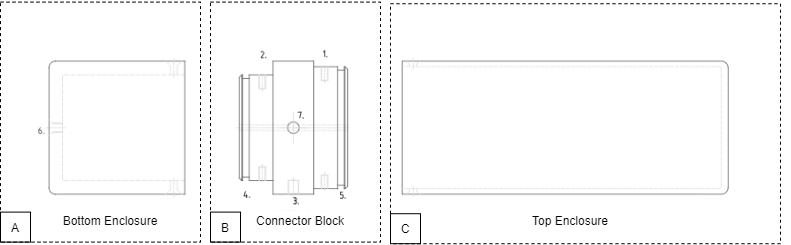
\includegraphics[width=\textwidth]{enclo_schem.PNG}
	\caption{2-D exploded view of the buoy enclosure showing (A) the bottom enclosure for the power module, (B) the connector block which also acts as a base for the electronics and (C) the top enclosure which covers the electronics. Drawn by R. Verrinder.}
	\label{fig:enclo_schem}
\end{figure}

\begin{table}[H]
	\centering
	\caption{Primary measurements of the buoy enclosure taken from the schematic in Appendex \ref{app:appendix.schem}}
	\setlength{\extrarowheight}{5pt}
	\begin{tabular}{l  l c}
		\hline
		\textbf{Component} &   \textbf{Dimension} &   \textbf{Size [mm]} \\
		\hline
		\hline
		\setlength{\extrarowheight}{2.5pt}
		\multirow{4}{*}{Top Enclosure} & Height & 240\\
		&  Outer diameter & 98  \\
		&  Wall thickness & 4 \\ 
		&  Base thickness & 5 \\
		\hline
		\multirow{3}{*}{Bottom enclosure} & Height & 100\\
		& Outer diameter & 98  \\
		& Wall and base thickness & 10 \\ 
		\hline
		\multirow{5}{*}{Connector Block} & Height & 80\\
		&  Outer diameter & 98  \\
		&  Top inner diameter & 89.94  \\ 
		&  Bottom inner diameter & 77.85\\
		&  O-ring thickness & 2.6 \\
		\hline
		\hline
	\end{tabular}
	
	\label{tab:enc_meas}
\end{table}

This design allows for easy access to the electronics as well as separation between the various subsystems. The connector block acts as a connection point for the electronics in version 1 of the buoy. This point of contact was a three-dimensional printed connector for a vertically mounted printed circuit board (PCB). In version 2 of the buoy, this was replaced by a row of screw holes around the connector block to connect a horizontal stack of customised PCBs. This was found to greatly improve the robustness of the system and prevented components from breaking during transport and deployment. The communication modules, microcontroller and sensors were mounted in the top enclosure while the batteries and power system were placed in the bottom enclosure. The power system was connected to the top enclosure through a drill hole in the connector block. The system was waterproofed by placing two o-rings on either side of the connector block. The top and bottom enclosure are fastened to the connector block using a a flat head counter-sunk hex screw. Finally a drill hole in the connector block allowed the system to be secured to the buoy stand preventing it from falling out during deployment.

\section{Electronics}

The electronics for the system refer to the communication subsystems, power electronics, sensors and processors. Due to project time constraints, the approach to developing the platform was to select off-the-shelf components that satisfied the subsystem specifications shown in Table \ref{tab:sys_specs}. Further consideration was given to components that were low power (SP011, SP012) and cost effective (SP013). Additionally, devices with intelligent operations were selected as this would allow us to effectively control the current consumption and operations of the device. These consisted of components with programmable settings such as digital sensors and modems. The following section gives an overview of the selection consideration for each subsystem.

\subsection{GPS}

A u-blox NEO-7M\footcite{UBLOX_M7N_DATA} GNSS reciever was initially selected during the 2018 design concept phase as it was easy to procure and has a small form factor. The positioning  module was designed around a Waveshare\footcite{waveshare} development board which significantly decreases the development time. The board comes with an active patch antenna which has a gain of about 30 dB \cite{waveshare}. In addition, the component is low power with a relatively fast acquisition time and accuracy. The device also can be configured to output diagnostic information such as dilation of procession with the associated measurement which can provide a greater understanding of satelite connectivity in the region. However,  this product has been depreciated by the time the latest buoy was developed. To overcome this, we opted for the u-blox NEO-M9N\footcite{UBLOX_M9N_DATA} module which had improved performance at a higher cost. Table \ref{tab:gps_mod} below shows a comparison of the two modules and their key performance parameters.

\begin{table}[H]
	\centering
	\caption{Comparison of key parameters between the initial u-blox NEO-7M GNSS module and the updated u-blox NEO-N9M module.}
	\label{tab:gps_mod}
	\setlength{\extrarowheight}{5pt}
	\begin{tabular}{l l l}
		\hline
		\textbf{Specification} & Neo-7M & Neo-M9N\\
		\hline
		\hline
		Positional accuracy [m] & 2.5  & 2.0 \\
		\hline
		\multirow{3}{*}{Communication type} & UART & UART\\ & I2C & I2C \\ & SPI & SPI\\
		\hline
		Cold-start time [s]& 30 & 26\\
		\hline
		Supply voltage [V] & 1.65 to 3.6 & 2.7 to 3.6\\
		\hline
		Active current draw [mA] & 32 &  42\\
		\hline
		Price & R269 \footnotemark & R1,195\footnotemark\\
		\hline
		\hline
	\end{tabular}
	\label{tab:neo7}
\end{table}
\footnotetext[1]{from Digikey \url{https://www.digikey.co.za/} ordered on 09/2020} 
\footnotetext{from Microrobotics \url{https://www.robotics.org.za/} ordered on 19/12/2018}
Table \ref{tab:gps_mod} shows the u-blox NEO-M9N offers improved performance  over the u-blox NEO-7M at a higher cost and higher power consumption. This module comes on a Sparkfun GPS Breakout - NEO-M9N U.FL (Qwiic) board which optionally comes with an integrated chip antenna. The chip antenna however has a very small gain making it unsuitable to be used for this application. Therefore, an additional antenna was bought. %TODO: name the antenna and link to the sparkfun board

\subsection{Iridium}

The Iridium modem is critical for ensuring data can be transmitted from remote locations. When selecting a modem, key considerations were given to the physical size, Bandwidth as well as coverage. In addition, we require a module that is low powered and cost effective. For this reason, we have selected the Rock block 9603 modem which has the following key specifications. This is a module that contains an Iridium 9603 modem on a specially -designed power board. The device communicates via UART with the option for flow control. The module contains a 10-pin picoblade. The module contains 4 communications pins, 1 digital input pin and 2 digital output pins for interfacing with. Power is supplied either through a 5V pin or 3.3V pin in addition to the ground pin. A brief description of the pin out is given in the table below: 

\begin{table}[H]
	\centering
	\caption{Pinout for the Rockblock 9603 Iridium Modem}
	\begin{tabular}{c l l}
		\hline
		Pin Number: & Label & Pin Description\\
		\hline
		\hline
		1 & RXD & UART Output Pin \\
		
		2 & CTS & Flow Control Clear To Send\\
		3 & RTS & Flow Control Request To Send\\
		4 & NetAv & Network Available \\
		5 & RI & Ring Inidcator \\
		6 & TXD & UART Input Pin \\
		7 & OnOff & Sleep Control\\
		8 & 5V & 5V max supply pin \\
		9 & Li-Ion & 3.7V max supply pin \\
		10 & GND & Ground \\
		\hline
		\hline
	\end{tabular}
	
	\label{tab:ir_pinout}
\end{table}

The device communicates via UART through the RXD and TXD pins. The CTS and RTS pins are optional if flow control is required. The OnOff pin can be used to put the device to sleep which significantly improves power performances. Finally, The NetAv and Ring Indicator are notification pins that can be used to indicate whether there is sufficient signal to transmit as well as to notify when a message is waiting to be downloaded respectively. 

Finally, the key characteristics for the device are shown in the table below:

\begin{table}[H]
	\centering
	\caption{Table showing key parameters and performance characteristics taken from the datasheet}
	\begin{tabular}{|c|c|}
		\multicolumn{2}{l}{Mechanical Features:}\\
		\hline
		\textbf{Antenna: } & Patch or External SMA\\
		\hline
		\textbf{Temperature Rating:} & -40ºC to +85ºC\\
		\hline
		\textbf{Dimensions}  & $45.0 \times 45.0 \times 15.0$ mm  \\
		\hline
		\textbf{Cost: } & R2,850.56\\
		\hline
		\multicolumn{2}{l}{Power Characteristics:}\\
		\hline
		\textbf{Supply Voltage} & 5v or 3.7v Li-Ion \\
		\hline
		\textbf{Start-Up Current} & 450mA \\
		\hline
		\textbf{Active Current} & 100mA \\
		\hline
		\textbf{Sleep Current} & 200uA\\
		\hline
		\multicolumn{2}{l}{Communication:}\\
		\hline
		\textbf{Baudrate} & 19200 b/s \\
		\hline
		\textbf{ Data bits} &  8\\
		\hline
		\textbf{Stop bits} & 1 \\
		\hline
		\textbf{Parity} & none \\
		\hline
		\textbf{Max Upload size} & 340 bytes \\
		\hline
		\textbf{Max Download Size} & 270 bytes \\
		\hline
	\end{tabular}
	
	\label{tab:ir_specs}
\end{table}

\subsection{Sensors}

2 versions of the buoy were developed from 2019 - 2020 with different sensing capabilities. The first version consisted of a DS18B20 Temperature sensor. This was a low cost, small form factor device that interfaced over One-wire. In version two, this was dropped in favour of the Bosh Sensortech BMP280 sensor. The BMP featured improved sensing capabilities, temperature compensation as well as a programmable interface. In addition, the sensor contains both an ambient temperature sensor as well as a pressure sensor. A comparison of each device is given in the table below

\begin{table}[H]
	\centering
	\caption{Comparison of performance between the BMP280 and DS18B20 environmental sensors.}
	\begin{tabular}{|c|c|c|}
		\hline
		& \textbf{BMP280} & \textbf{DS18B20} \\
		\hline
		Temperature Range & $-40^\circ C \text{ to } 85^\circ C$&$-55^\circ C \text{ to } 125^\circ C$ \\
		\hline
		Accuracy & $1^\circ C \text{ for } T < 0^\circ C$ & $1^\circ C \text{ for } T < 0^\circ C$ \\
		\hline
		Pressure Range  & N/A & 300 to 1100 HPa \\
		\hline
		Pressure Accuracy & N/A & 1.7 HPa $ \text{ for } T < 0^\circ $\\
		\hline
		Price & R87,84 & R85.17 \\
		\hline
	\end{tabular}
	\label{tab:senv_spec}
\end{table}

The BMP 280 is a chip that can be ordered standalone or comes on a I2c/SPI ready breakout board. The device on a breakout board is cheaper than than DS18B20 and can measure both temperature and Pressure whereas the DS18B20 can only measure temperature. The Power characteristics of each device are given in the table below

\begin{table}[H]
	\centering
	\caption{Comparison between supply voltage and current draw of the BMP280 and DS18B20}
	\begin{tabular}{|c|c|c|}
		\hline
		&  \textbf{BMP280} & \textbf{DS18B20}\\
		\hline
		Supply Voltage & 3.0V - 5.5V & 1.71V - 3.6V\\
		Sleep Current & $0.75\mu A$ & $0.3\mu A$\\ 
		Active Current & $1500\mu A $ & $4.2\mu A$\\
		\hline
	\end{tabular}
	
	\label{tab:env_power}
\end{table}

The BMP280 was chosen for its comparable performance and accuracy. In addition, the BMP280 features more sensing capabilities and is more power efficient and cost effective than the DS18B20 making it suitable for this application.\par 

Finally, a digital sensor for power monitoring was selected to provide constant feedback on the status of the power system. This will be used to monitor the battery voltage as well as the current draw to make sure that the system does not deplete the energy reserves to quickly. To achieve this a INA219A IC was selected and mounted on a custom PCB with a shunt resistor of known resistance. The device has a high reported accuracy of 1\% over a full temperature range and is fully programmable. The device  communicates via I2C with 16-bit registers storing ADC values for  Current (mA),Voltage (V) as well as power (mW). The device is extremely low power with a high voltage measurement range and on-board calibration features. Some key performance parameters are shown in the table below:

\begin{table}[H]
	\centering
	\caption{Performance specifications for the INA219 current monitor chip.}
	\begin{tabular}{|l|l|}
		\hline
		\textbf{Operating Temperature: }& $-40\degree C\text{ to } 125\degree C$ \\
		\hline
		\textbf{$V_{shunt}$ range: }& $40mV \text{ to } 320mV$\\ 
		\hline
		\textbf{$V_{bus}$ rage: } & $0V - 16V \text{ or } 0V-32V$\\
		\hline
		\textbf{ADC Resolution: } & 12-bits\\
		\hline
		\textbf{Measurement Error: } &$\pm 1\%$\\ 
		\hline
		\textbf{Price: } & R17.77\footnotemark\\
		\hline
		\multicolumn{2}{l}{Power Characteristics}\\
		\hline
		\textbf{Supply Voltage: } & $3.3V \text{ to } 5V$\\
		\hline
		\textbf{Quiescent Current: } & $0.7mA \text{ to } 1mA$\\
		\hline
		\textbf{Standby Current: } & $6\mu A \text{ to } 15\mu A$\\
		\hline
	\end{tabular}
	
	\label{tab:INA_spec}
\end{table}
\footnotetext{source: \url{https://www.digikey.co.za/}}

\subsection{Inertial Measurement Unit}

The MPU6050 is a 6-axis IMU that measures the acceleration and rotational velocity of 3 axes respectively.This component has a small form factor, low power and is fully programmable allowing the device to operate in different modes thereby optimising the data flow to and from the device. While the device does not contain a magnetometer, this is not an issue since the region suffers greatly from magnetic distortion \cite{kohout2015device} thereby rendering all readings to be unreliable. In addition, The acceleration of waves can be defined by the stoke supper limit \cite{kohout2015device} as 0.5g for a non breaking wave. The device has a programmable full scale range for both the accelerometer and gyroscope. IT contains an IIR filter and on-board self testing for added robustness and data integrity thereby making it  the ideal device for this application. The key parameters for the device are shown in the table below:
\begin{table}[H]
	\centering
	\caption{Performance Characteristics of the MPU6050 6-axis IMU }
	\begin{tabular}{|l|l|}
		\multicolumn{2}{l}{Accelerometer:}\\
		\hline
		Full Scale Resolution:  & $ \pm 2g \text{ to } \pm8g$\\
		\hline
		Sensitivity: &  $61.17 \mu g/LSB^{-1} \text{ to } 488.281\mu g/LSB^{-1}$\\
		\hline
		Sample Rate: & 4Hz - 1000Hz\\
		\hline
		Noise Performance: & $400\mu g/\sqrt{Hz}$\\
		\hline
		\multicolumn{2}{l}{Gyroscope:}\\
		\hline
		Full Scale Resolution:  & $\pm 250\degree/s \text{ to } \pm 2000\degree/s $ \\
		\hline
		Sensitivity: &  $7.63(\mu\degree/s)/LSB^{-1} \text{ to } 60.98(\mu\degree/s)/LSB^{-1}$\\
		\hline
		Sample Rate: & 4Hz - 8000Hz\\
		\hline
		Noise Performance: & $0.005(\mu\degree/s)/\sqrt{Hz}$\\
		\hline
		\multicolumn{2}{l}{Device Characteristics:}\\
		\hline
		Temperature Range: & $40\degree C \text{ to } 85 \degree C$\\
		\hline
		Low Pass Filter Range: & 5Hz to 256Hz \\
		\hline
		Supply Voltage: & 2.375V to 3.46V\\
		\hline 
		Active Current: & 3.9mA (Max) \\
		\hline
		Low Power Current: & $< 20 \mu A$ for $ODR < 5Hz$\\
		\hline
		Cost: & R40.00 \footnotemark\\
		\hline
	\end{tabular}
	\label{tab:mpu_specs}
\end{table}
\footnotetext{Source: \url{https://www.communica.co.za/}}

The device has a high range for both gyroscope and imu with ideal low power performances making it the ideal device. In addition, the device comes prototype ready on the GY-521 development board. The device can be interfaced either using SPI or I2C. For this application, the device was interfaced with using I2C.

\subsection{Memory}

Physical memory is an important feature in the device as it allows for permanent storage of data during the life cycle of buoy. Having the device in various sleep modes may result in lost data if the data is stored in RAM.

Flash Chips were selected as a permanent Solution. An array of 4 AT45DB641E SPI Serial Flash Chips were selected and mounted on a PCB directly interfacing with the system. Each chip can hold up to 64Mbit of data. Data can be read/ written at speeds of up to 85MHz of 15MHz in low power mode. The device is low power with high data retention requiring a supply voltage of 1.7V – 3.6V and draws a maximum of 11mA in Active Read mode thereby making it one of the lowest power consumption components in the system. In addition, the device comes with 2 x 256byte buffers that can store data while a read/ write operation is taking place. Memory is Organized into sectors (2 – 256 Kbs long), blocks (2kB long) and pages (256 bytes) with write, read and erase options at each level. The following table shows key performance characteristics

\begin{table}[H]
	\centering
	\caption{Key performance characteristics for the AT45DB641E flash chips.}
	\begin{tabular}{|l|l|}
		\hline
		Operating Temperature:  & $ -40\degree \text{ to }85 \degree$ \\
		\hline
		Storage Capacity: & 64 Mbit \\
		\hline
		Supply Voltage    & 1.7V -3.6V\\
		\hline
		Standby Current: & $45\mu A$ \\
		\hline
		Active Current:  & $22mA$ \\
		\hline
		Unit Cost:       & R 65.307 \footnotemark\\
		\hline
	\end{tabular}
	
	\label{tab:flash_specs}
\end{table}
\footnotetext{Source: \url{https://za.rs-online.com/}}
\subsection{Processor}

For the processor, a single processing unit was selected to reduce complexity of the system. However, in order to satisfy the requirements for the buoy, a processor must be selected with sufficient peripheral ports to handle communication from all sensors, communication modules and memory banks. In addition, there should be sufficient digital input and output pins to control the sensors and provide feedback The communication peripheral requirements are condensed into the following table: 

\begin{table}[H]
	\centering
	\caption{ Type and number of communication ports in order to facilitate communication with  all the external modules.}
	\begin{tabular}{|l|l|}
		\hline \hline
		Peripheral Name: & Qty \\
		\hline \hline
		UART & 2\\
		I2C & 2\\
		SPI & 2\\
		Digital Pins & 11\\
		\hline 
	\end{tabular}
	\label{tab:micro_ports}
\end{table}

Additionally, the processor needs to have a high resolution and large memory bank to handle incoming data. For this reason, a 32-bit micro-controller was identified as the ideal component for the processing system. 3 processors were selected from the STM32 range of microcontrollers and prototyped at various phases during the development cycle. The first version of the buoy contained the STM32F407 which is available on a 100-pin development board thereby decreasing the development time and increasing the technology readyness level of the system. This device was found to have more peripherals than required and had a large power requirement. Therefore the device was replaced by the STM32F446-RE which had significantly reduced peripherals and more optimal performance. The final processor selected was the STM32l476RG. Which matched the STM32F446 in pinout and peripheral however it was significantly more optimised for low power operation. The device had significantly more wake up pins with an extremely low power consumption therefore being the optimal choice. In addition, the development board for the STM32l476 has an on-board debugger which can be removed to reduce the physical size of the device. The STM32L4 can also be configured to passively detect a brownout event as well as a low power event which provides critical feedback regarding the device's performance. Some key performance parameters of the STM32l476 are shown in the table below:

\begin{table}[H]
	\centering
	\caption{Performance parameters for the STM32L4 microcontroller. }
	\begin{tabular}{|l | l|}
		\multicolumn{2}{l}{Electrical Characteristics:}\\
		\hline
		\textbf{Input Voltage: }    & $1.71V \text{ to } 3.6V$ \\
		\hline
		\textbf{Active Current Draw: }    & $100 \mu A/Hz$ \\
		\hline
		\textbf{Shutdown Mode Current Draw: }    &  $30nA$ \\
		\hline
		\textbf{Standby Mode Current Draw: }    &  $420nA$ \\
		\hline
		\textbf{$V_{brownout}$ Threshold:} &  $1.66V \text{ to } 2.90V$\\
		\hline
		\multicolumn{2}{l}{Computational Characteristics:}\\
		\hline
		\textbf{Processor: }    &  ARM Cortex-M4 \\
		\hline
		\textbf{MCU Size: }     & 32-bit\\
		\hline
		\textbf{Float representation: } & Hardware FPU \\
		\hline
		\textbf{Flash size: } & 1MB\\
		\hline
		\textbf{RAM Size:} & 128 KB\\
		\hline
		\textbf{Clock Source: } & LSE, HSE, LSI, MSI, HSI \\
		\hline
		\textbf{System Clock Frequency: } & 4MHz to 80MHz \\
		\hline
		\textbf{Dhrystone Benchmark: } & 1.25 DMIPS/Hz \\
		\hline
		\multicolumn{2}{l}{Communication Ports:} \\
		\hline
		\textbf{Total  Communication ports: } & 20 \\
		\hline
		\textbf{UART Ports} & 5 \\
		\hline
		\textbf{I2C Ports} & 3 \\
		\hline
		\textbf{SPI Ports} & 3 \\
		\hline
	\end{tabular}
	
	\label{tab:stm_spec}
\end{table}

The STM32l4 also features seven general purpose timers as well as two advanced timers and two low power timers. In addition, the device has five wake up pins which allow the device to be woken up from deep sleep (shutdown) via an external source. The device is capable of DSP processing using external libraries provided by the manufacturer and a real-time clock thereby making it the ideal component to be a processor for the buoy.

\subsection{Power Electronics}

Based on the aforementioned Hardware selection, the following power requirements are outlined in the table below:

\begin{table}[H]
	\centering
	\caption{Current consumption of various components as well as the estimated maximum possible current draw}
	\begin{tabular}{|c|c |c|c|}
		\hline
		Device Name & QTY &  Supply Voltage & Maximum current Draw\\
		\hline
		Ublox NEO-M9N & 1 & 3.3V & 42mA \\
		\hline
		Rockblock 9603 & 1 & 5V &  450mA\\
		\hline
		BMP280 & 1 & 3.3V & 0.0042mA\\
		\hline
		INA219A & 1 & $V_{Bat}$ & 1mA\\
		MPU6050 & 1 & 3.3V & 3.9mA\\
		\hline 
		AT45DB641E & 4 & 3.3V & 88mA\\
		\hline
		STM32L476RG & 1 & 5V & 2.6mA\\
		\hline
		\cline{4-4}
		\multicolumn{2}{c}{} &\multicolumn{1}{c}{\textbf{total:}} & \multicolumn{1}{c}{587.50mA} \\
		\cline{4-4}
		\cline{4-4}
	\end{tabular}
	
	\label{tab:pow_budget}
\end{table}

From table \ref{tab:pow_budget} we can expect a maximum current draw of 587.50. The largest consumer of power is the Rock-block 9603 which can draw up to 450mA when charging. Therefore, the power supply needs to be able to supply at-least 500mA during start up. Current can be conserved by placing the devices into sleep mode which further reduces the current consumption from the batteries. Finally, By only turning the components on when required, even less power can be conserved. \par 

Therefore, a regulator is required that is capable of supplying the required current  while being able to stand the drastic changes in current consumption. A decision was made to use a 5V low Dropout regulator to supply the 5V components directly i.e. the iridium modem and the micro-controller. The 3.3V components are powered through the on-board 3.3V regulator for the STM32L4 nucleo development board. The Low Dropout regulator is a LP3876 7V LDO capable of supplying up to 3A. The device has a quick response to step changes and an adjustable output voltage thereby making it the ideal device to supply power. The output voltage level can be controlled by selecting capacitors. For this application a $10 \mu C$ tantalum capacitor was used as tantalum capacitors have  excellent robustness and transient responses especially at low temperatures.  Some key characteristics for the device are given in the table below

\begin{table}[H]
	\centering
	\caption{Key Performance Characteristics for the LP3876 Low Dropout Regulator}
	\begin{tabular}{|l|c|}
		\hline
		Input Voltage & $2.5V \text{ to } 7.0V$  \\
		\hline
		Voltage Regulation (over current)& 0.14\%\\
		\hline
		Dropout Voltage at 3A & 0.8V to 1.2V  \\
		\hline
		Quiescent Current at 3A &  14mA\\
		\hline
		Temperature Range & $-40 \degree C \text{ to }125 \degree C$\\
		\hline
		Unit Cost & R95.19 \footnotemark\\
		\hline
	\end{tabular}    
	\label{tab:lp_spec}
\end{table}

\footnotetext{source: \url{https://www.digikey.co.za/}}

The LDO was placed on a customised PCB  with the INA 219 Current sensor as well as an indicator LED to show that the batteries have sufficient charge. The power board was supplied by 3.6V C-cell LiSOCl2 batteries. These batteries have ideal low temperature characteristics as well as a high capacity. 2 cells were placed in series to create a 7.2V power source which was placed in parallel with another 7.2V array to increase the capacity. The batteries, battery holders and power board are connected to form a single subsystem which was placed in the bottom enclosure and connected to the micro-controller via a 7-pin cable.

\section{Final Assembly}
\label{sec:ch3_final_assembly}
The final electronics choice and configurations are shown in the figure below:

\begin{landscape}\centering
	\vspace*{\fill}
	\begin{figure}[htpb]
		\centering
		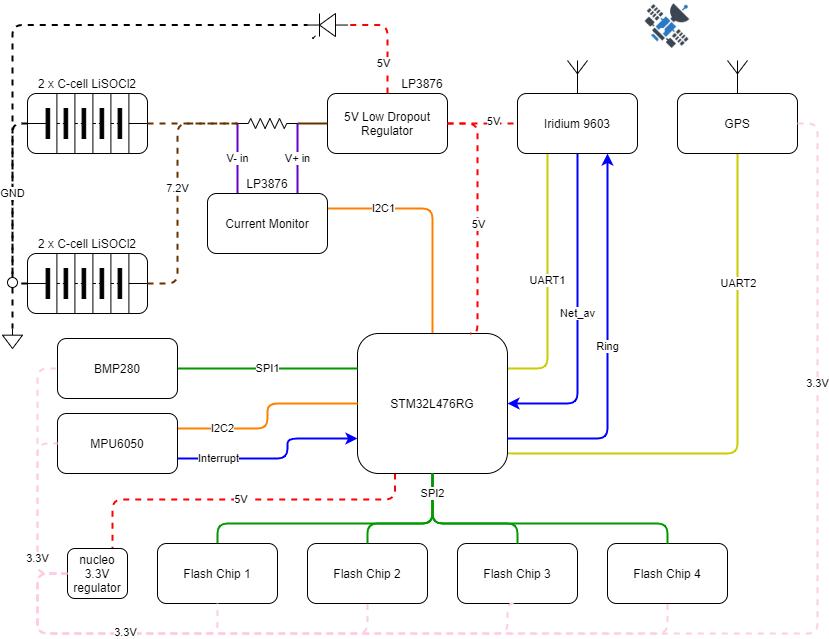
\includegraphics[height=0.6\textheight, width=1.2\textwidth]{figs/SHARC_Final.png}
		\caption{Simplified schematic of the final version of SHARC buoy showing power supply (dash), communication (solid) and digital connections (arrows) and configurations}
		\label{fig:sharc_final}
	\end{figure}
	\vfill
\end{landscape}


A final costing of the system is provided in the table below:
\begin{table}[H]
	\centering
	\caption{Approximate procurement cost for a single SHARC buoy node.}
	\begin{tabular}{l c r r}
		\hline \hline
		\textbf{Component Name:} & \textbf{QTY:} & \textbf{Unit Cost} & \textbf{Total:}  \\
		\hline \hline
		Buoy Enclosure and Stand  & 1 & R1,206.84 & R1,206.84 \\
		Ublox Neo-M9N & 1 &  R1,195.45 &R1,195.45\\
		Rockblock 9603 & 1 & R3,278.144 & R3,278.144 \\
		M1621HCT Helical Antenna & 1 & R1,411.15 & R1,411.15 \\
		BMP280 & 1 & R46.00 & R46.00 \\
		INA219A & 1 & R17.77 & R17.77 \\
		MPU6050 & 1 & R40.00 & R40.00 \\
		AT45DB641E & 4 & R65.307 & R261.229 \\
		Nucleo-l476RG & 1 & R215.98 & R215.98 \\
		Fanso C-cell 9000mAh Battery & 4 & R101.81 & R407.24 \\
		BHC-2ND Battery Holder & 4 & R61.87 & R247,48 \\
		LP3876 5V regulator & 1 & R95.19 & R95.19 \\
		Wiring and Connectors & - & R136.46 & R136.46 \\
		\hline 
		\hline
		& & \textbf{ Grand Total: } & R8,421.13\\ 
		\hline \hline
	\end{tabular}
	\label{tab:total_cost}
\end{table}

Customised PCBs were designed to connect the various subsystems together. The device was kept modular by separating PCBs and grouping devices by functionality. A circuit board was created for the Dropout regulator and INA219 current sensor which was affixed to 4 x C-cell battery holders.The battery holders have leads which were were arranged in a 2-series, 2- parallel configuration.

\begin{figure}[H]
	\centering
	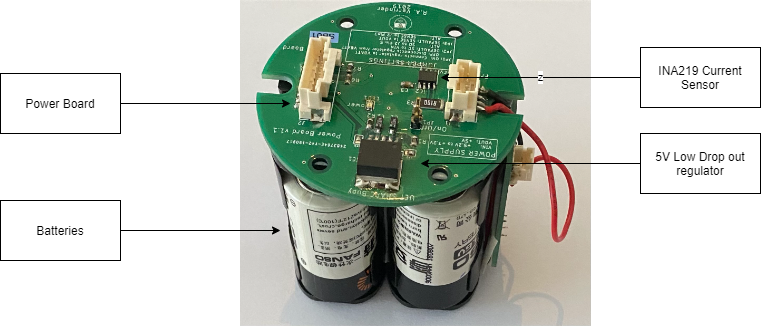
\includegraphics[scale = 0.5]{bot_encl.png}
	\caption{Power Module for the SHARC BUOY. A custom PCB with Dropout Regulator and current sensor connected to a battery pack}
	\label{fig:bot_elec}
\end{figure}

This module was placed in the bottom enclosure and fastened to the connector block using a hex screw. A customised 7-pin duraclick cable connects the module to the modules in the top enclosure. A main connector board was developed with duraclick connections for each of the aforementioned devices. The board contains 2  2x16 female header rows to fit the morpho connectors of the nucleo-l4 development board. 2 more disc-shaped PCBs were developed. First a communication boards which contains a 4-pin female header to connect the ublox GPS module and 2 brackets to mount the iridium module vertically. A helical antenna connects to an SMA antenna on the Iridium module. Then a sensor board for the IMU and environmental sensor. The boards were connected in a stack configuration and fastened to the connector block using M6 metal Hex Spaces with the communication board being placed at the top for direct line of sight with satellites. The environmental board was secured to the base of the connector block with the BMP280 placed face-down over a hole drilled through the connector block allowing it to interface with the environment.
\begin{figure}[H]
	\centering
	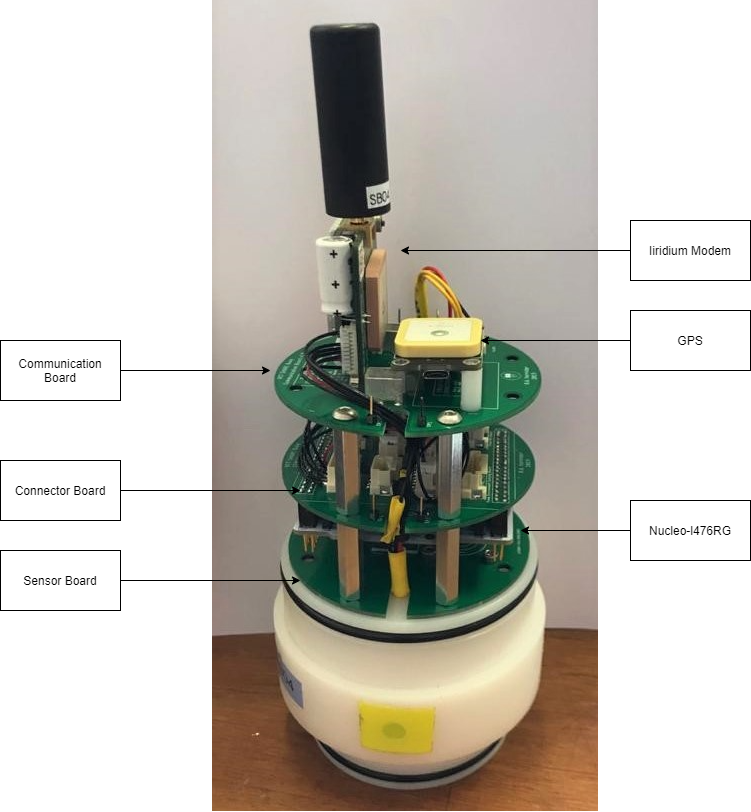
\includegraphics[scale =0.5]{Top_encl.png}
	\caption{Electronic Stack for the top module consisting of connector board, micro-controller board and sensor board attached to the connector block }
	\label{fig:top_elec}
\end{figure}

This configuration greatly increases the robustness of the electronics and can overcome breaking caused by poor handling or improper deployment.  The top enclosure is placed over the electronics and fastened to the connector block using Hex screws. Finally, the system is placed in the stand housing and secured using another hex screw.

\begin{figure}[H]
	\centering
	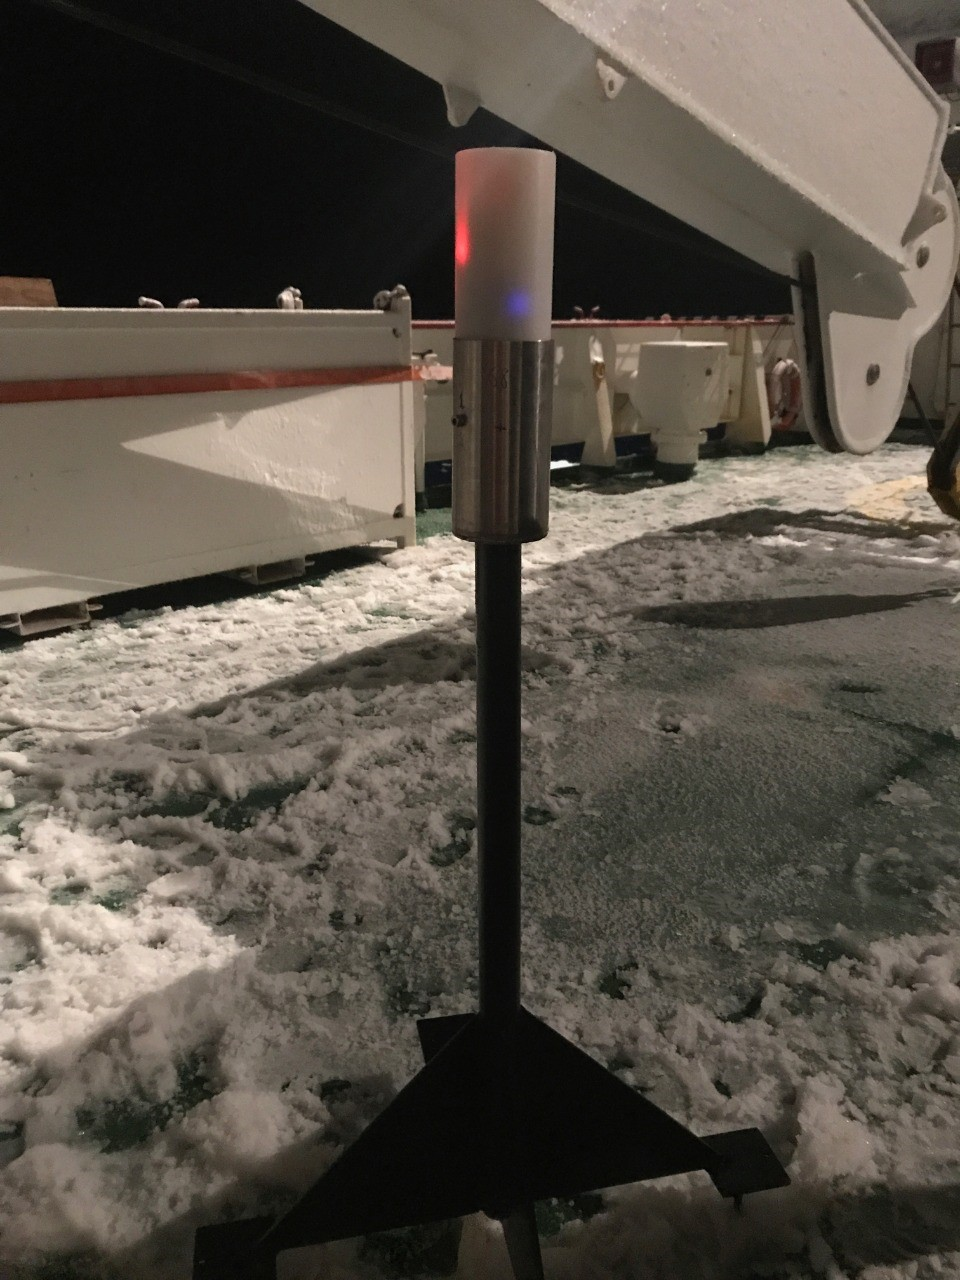
\includegraphics[scale = 0.5]{full buoy.jpg}
	\caption{SHARC BUOY fully assembled and in deployment state. Electronics placed in enclosure and fastened to the buoy stand. LEDs on the various components indicate that the device is in working order}
	\label{fig:my_label}
\end{figure}
